\documentclass[letter, 10pt]{article}
\usepackage[utf8]{inputenc}
\usepackage[spanish]{babel}
\usepackage{amsfonts}
\usepackage{amsmath}
\usepackage{graphicx}
\usepackage{url}
\usepackage{hyperref}
\usepackage[top=3cm,bottom=3cm,left=3.5cm,right=3.5cm,footskip=1.5cm,headheight=1.5cm,headsep=.5cm,textheight=3cm]{geometry}


\begin{document}
\bibliographystyle{plain}
\pagestyle{empty}

\title{Taller de Modelos y Métodos Cuantitativos \\ \begin{Large}Estado del Arte: ``Car Sequencing Problem''\end{Large}}
\author{Cristián D. Maureira Fredes}
\date{\today}
\maketitle

\section{Introducción}
\label{sec:introduccion}
\frame
{
\frametitle{Introducción}
\begin{itemize}
	\item Motivación del problema.
	\item Sobre la técnica.
	\item Implementación inicial.
	\item Sintonización.
	\item \blue{Control}.
	\item Resultados.
\end{itemize}
}



\section{Definición del Problema}
\label{sec:definicionProblema}
%Descripción del problema, su complejidad, en que consiste, cuales son sus objetivos,
%restricciones, variantes más conocidas. 

El \emph{Car Sequencing Problem} es un problema de satisfacción de restricciones (CSP), posee la
característica de ser NP-duro~\footnote{
NP-duro es el conjunto de los problemas de decisión que contiene los problemas H
tales que todo problema L en NP puede ser transformado polinomialmente en H.
Esta clase puede ser descrita como conteniendo los problemas de decisión que son
al menos tan difíciles como un problema de NP.}
, además corresponde a un tipo de variación del problema NP-completo \emph{Job-Shop Scheduling}.%,
%pero con un uso de razonamiento automatizado, es decir, con un enfoque dedicado a estudiar y comprender
%diferentes características del razonamiento, permitiendo así construir programas que le den la posibilidad
%a los computadores para razonar en forma autónoma.
 
Siguiendo la misma idea, es válido señalar que el \emph{Car Sequencing Problem} es un tipo de problema de planificación
de tareas en una línea de ensamblaje de autos, donde cada uno es perteneciente a un clase de automóvil, debido al conjunto
de opciones y accesorios que posee (airo acondicionado, centralizado eléctrico, etc), y cada una de las opciones o
accesorios se instala en una planta distinta, por lo que el objetivo principal es el poder encontrar el orden en la
secuencia de los vehículos, preocupándonos de no exceder la capacidad de cada planta de ensamblaje y también cumplir con la demanda.

Por lo tanto, si realizamos una definición más formal de nuestro problema, podríamos decir lo siguiente:
Teniendo una lista de vehículos dada, cada uno con sus respectivas opciones requeridas,
necesitamos establecer un orden en la línea de ensamblaje, con el fin de que cada subsecuencia de $q$ vehículos
tengamos a lo más $p$ que requieren de una determinada opción. Es importante tener en consideración que los
valores de $p$ y $q$ están asociados a cada opción de los vehículos.

Con respecto a la información que el problema otorga, podemos decir que contamos con:
\begin{itemize}
	\item Cantidad de vehículos de cada tipo o clase a producir (demanda)
	\item Lista de las opciones con la cual se constituye cada tipo o clase de vehículo, la cual puede utilizar una representación
		booleana para saber si cierto tipo de automóvil posee o no una determinada opción.
	\item Capacidad de las plantas que se preocupan de instalar la determinada opción.
\end{itemize}

Nuestro objetivo principal es:
\begin{itemize}
	\item Encontrar un orden en nuestra secuencia, que sirva para minimizar el costo por cada restricción insatisfecha.
\end{itemize}

Con respecto a las restricciones, tenemos que:
\begin{itemize}
	\item En cada subsecuencia de los $q$ vehículos, a lo más pueden haber $p$ que requieran de la opción determinada.
		Donde $p$ y $q$ son valores asociados a cada opción.
	\item La capacidad de cada planta de ensamblaje no puede ser excedida, es decir, cumplir con la demanda de cada automóvil
		sin abusar de una planta determinada.
	\item Por cada tipo de auto, el numero de autos de ese tipo debe ser secuenciado, es decir, todos los automóviles de cada clase
		deben estar presente en una secuencia determinada.
\end{itemize}





\subsection{Estado del arte problema}
\label{sec:estadoArte}
%Debe contener: técnicas usadas en su resolución (en general las que han sido mas
%efectivas a la fecha), mejores resultados, estrategias mas usadas en su resolución,
%representacion, movimientos, penalización, etc..


El \emph{Car Sequencing Problem}~\cite{parello} es presentado por primera vez en la \emph{Journal of Automated Reasoning},
del año 1986 en \emph{EEUU}, por \emph{B.D Parello}, \emph{W.C. Kabat} y \emph{L. Wos}, siendo una variación
del problema ya conocido en el área de la Inteligencia Artificial, como lo es el \emph{Job-Shop scheduling problem},
pero usando otro tipo de razonamiento, el \emph{Razonamiento automatiza}, de ésta manera logran enfocar su trabajo
en el problema que ocurre en las líneas de producción de automóviles.

Desde la publicación del presente problema hasta los últimos años, han aparecido en distintas conferencias a lo largo
del mundo, diferentes formas de atacar el problema, que nos llevan desde  ``programación lineal'', ``Evolutionary Approaches''
y ``Local search'' con sus variantes.

Las técnicas que han sido utilizadas hasta el momento, no han sido desarrolladas sólo por matemáticos, sino que por una amplia
gama de investigadores, que van desde científicos del área de la producción, física, biología y gestión.

No obstante, gracias a los avances que ha tenido el campo de la Inteligencia Artificial, han aparecido nuevas metodologías,
que se relacionan con otras áreas como lo son la computación evolutiva, genética,  redes neuronales, neurofisiología;
los cuales han realizado contribuciones importantes a los problemas que tienen que ver con la ``planificación'' (scheduling).
Lo anteriormente señalado afirma el hecho que los problemas relacionados con la ``planificación'' abarcan muchas áreas en el mundo,
y que los trabajos en dicha área no tienen que ver sólo con científicos computacionales.

A continuación se describen algunos de los métodos más importantes que han sido propuestos desde el año
en que el \emph{Car Sequencing Problem} fue dado a conocer en el mundo de la investigación científica.


\subsection{Acercamientos heurísticos}
Existen distintos acercamientos que se han propuesto, que tienen como objetivo principal
encontrar una solución óptima lo más rápido posible.
Los acercamientos descritos a continuación son \emph{búsqueda local (local search)},
\emph{greedy approach}, \emph{Ant colony Optimization} y por último, \emph{Algoritmos genéticos}

\subsubsection{Búsqueda Local (Local Search)}
La \emph{Búsqueda Local} puede ser utilizada en distintos problemas que se formulan
de una forma determinada para poder encontrar una solución que maximice un criterio alrededor de un número
de soluciones candidatas

Lo que hace la \emph{Búsqueda Local}, es moverse en su vecindario solución por solución en el espacio previamente establecido
de las soluciones candidatas, también conocido como espacio de búsqueda, hasta que una solución considerada \emph{óptima}
es encontrada ó se termina el plazo de tiempo para encontrar la solución, por otra parte, 
el vecindario va a estar definido netamente con respecto al modelamiento del problema.

Actualmente existen variadas aproximaciones propuestas sobre \emph{Búsqueda Local},
para resolver el presente problema.
La diferencia aquí, es que la mayoría de las propuestas son acercamientos más
genéricos, es decir, se han utilizado varios problemas para aplicar la propuesta
planteada y entre ellos se encuentra el problema en cuestión, como por ejemplo~\cite{DTWZ94}
que nos plantea una mejora en el sentido de una \emph{Estrategia de Búsqueda}, considerando
el conflicto mínimo con respecto a la heurística \emph{hill-climbing}~\footnote{
Técnica de optimización matemática, puede ser usada para resolver problemas con muchas soluciones.
Consiste en escoger una solución aleatoria (potencialmente no óptima) y comienza a
realizar pequeños cambios a dicha solución en cada iteración, en cada momento se va mejorando un poco más.
}
y ha propuesto un escape con respecto a los mínimos locales incrementando el peso de las
restricciones que no se cumplen.

Por otra parte existen otras propuestas que se han enfocado netamente en resolver éste problema,
como es el caso de ~\cite{PG02}, que considera los algoritmos de \emph{Búsqueda local}
que se basan en una representación de una permutación y la evaluación de las restricciones que no se
cumplen utilizando funciones de penalización.

De la misma forma tenemos el caso de lo que plantea Gottlieb et al. en \cite{GPS03}, quien se refiere
a una parte en especial de nuestro problema, la construcción de la secuencia inicial, por lo tanto
sabemos que en la mayoría de los casos, la secuencia inicial de vehículos, de donde parte la
\emph{Búsqueda Local}, es una permutación aleatoria de un conjunto de vehículos para comenzar
a ensamblarlos, sin embargo la propuesta nos señala el construir ésta secuencia inicial en una forma
\emph{Voraz (Greedy)}~\footnote{
se refiere a a realizar una elección del siguiente elemento considerando una función heurística de optimización,
con la esperanza de llegar a una solución general óptima.
}
, lo que queda claramente demostrado en dicha publicación,
debido a las grandes mejoras en el proceso de solución.

\subsubsection{Acercamiento Voraz (Greedy approaches)}
Teniendo en consideración el \emph{Car Sequencing Problem}, podemos construir una secuencia
en una forma \emph{Voraz (Greedy)}, eligiendo el siguiente vehículo de la secuencia
considerando una función heurística de optimización.
El primero acercamiento utilizando \emph{Greedy} fue propuesto por
Hindi and Ploszaski en 1994~\cite{HP94}. Volviendo al procedimiento anteriormente descrito, la idea
central que nos plantea Gottlieb et al. en \cite{GPS03}. Claramente, ahora la elección que podemos
realizar en cada paso de nuestro algoritmo, debe ser la más óptima, en otras palabras,
elegir el vehículo que posea el menor número de restricciones no satisfechas.

Matemáticamente hablando, podríamos decir lo siguiente:
Dado una secuencia parcial $\pi$, el siguiente vehículo es seleccionado entre los vehículos $c_j$
que minimice la siguiente función,
$$newViolations(\pi, c_j) = \sum_{o_{i}\in O}r(c_j,o_i)\cdot violation(lastCars(\pi\cdot <c_j>,q(o_i)),o_i)$$
donde $o_j$ es una opción del vehículo $c_j$ y donde $lastCars(\pi',k)$ es la secuencia compuesta de los
últimos $k$ vehículos de $\pi'$, si $|\pi'| \geq k$, en otro caso $lastCars(\pi' , k) = \pi')$.

El problema acá, es que por lo general, el conjunto de vehículos seleccionados que minimizan la función
$newViolations$, contiene más de un auto, por lo tanto acá viene otra decisión importante. ¿Cuál de esos
autos elegimos?, por lo que Gottlieb et al.~\cite{GPS03} nos señala que es necesario utilizar otra técnica heurística para 
romper dicha incertidumbre, de la misma forma propone 6 heurísticas distintas. La heurística que presente
un mejor desempeño es llamada \emph{``dynamic sum of utilization rates''}, la cual consta en que en cada paso
añadimos el vehículo que maximiza la suma de las tasas de uso de opciones necesarias, estas tasas de uso se actualizan
dinámicamente cada vez que añadimos un nuevo auto al final de la secuencia.

\subsubsection{Ant Colony Optimization (ACO)}
El algoritmo \emph{Ant Colony Optimization (ACO)}, tal como es descrito en \cite{DS05},
toma su inspiración en el comportamiento de ciertas especies de hormigas. La idea central
es notar que las hormigas depositan en el suelo una feromona, con el objetivo de marcar
un camino favorable para que los otros miembros de su colonia puedan seguirlo. Por lo tanto
\emph{ACO} busca aplicar un mecanismo similar para resolver problemas de optimización.

En otras palabras, \emph{ACO} es una forma de modelar cierto problema de tal forma
que busquemos siempre el camino con mínimo costo en un grafo determinado, y por supuesto,
utilizar \emph{hormigas artificiales} para buscar los caminos que más nos pueden favorecer.


El primer algoritmo de \emph{ACO} fue propuesto por Christine Solnon~\cite{Sol00},
y se trata de resolver un problema de satisfacción de restricciones de permutación~\footnote{
El objetivo principal es poder encontrar la permutación de $n$ valores conocidos,
para asignarlos a $n$ variables, bajo ciertas restricciones.
},
utilizando el concepto de \emph{hormigas artificiales}. Principalmente está diseñado
para resolver un problema general de combinatoria.

En enfoque que entrega el trabajo previamente señalado~\cite{Sol00} con respecto
al \emph{Car Sequencing Problem} es el siguiente:
Recordando nuestro problema principal, sabemos que consiste
en realizar la óptima planificación de los vehículos en una línea de ensamblaje,
donde tenemos $n$ vehículos para producir, que están agrupados en $k$ tipos
de autos~\footnote{
Cada conjunto de autos de un mismo tipo tienen las mismas opciones
}, y sabemos también que cada opción $i$ está asociada con una restricción de capacidad
representada por una tasa $p_i/q_i$, que especifica que para cualquier secuencia
de $q_i$ autos consecutivos en le línea de ensamblaje, tenemos al menos $p_i$ vehículos
que requieren dicha opción.
Finalmente el objetivo será encontrar una permutación de $n$ vehículos que satisfacen
todas las restricciones de capacidad, tomando en consideración que nuestra feromona
se pondrá sobre las parejas de los vehículos consecutivos con el fin de aprender
las sub-secuencias de vehículos más prometedoras (óptimas).

No conforme con el desempeño mostrado en el trabajo anterior, Gottlieb et al.~\cite{GPS03}
proponen un nuevo algoritmo que introduce tres nuevas mejoras:
\begin{itemize}
	\item Se utiliza una estrategia elitista, por lo que la feromona es usada para romper el lazo entre los mejores vehículos solamente.
	\item Se integran mejoras del trabajo ~\cite{Stu}, para favorecer la exploración.
	\item Se usan funciones heurísticas de tipo \emph{voraz (greedy)} para guiar las hormigas.
\end{itemize}
Con las mejoras anteriormente planteadas se logra obtener un resultado mucho más óptimo computacionalmente.

\subsubsection{Algoritmos Genéticos (Genetic Algorithms)}
Los \emph{Algoritmos Genéticos} son una técnica computacional que tienen como objetivo principal,
el encontrar una solución exacta o aproximada en problemas de optimización y búsqueda.

En el trabajo de Warwick y Tsang~\cite{WT95} se propone un algoritmo genético especialmente
para resolver el \emph{Car Sequencing Problem} que se diferencia de los algoritmos genéticos
tradicionales pues ingresa ciertas características especiales como el \emph{elitismo}~\footnote{
proceso de seleccionar mejores individuos, seleccionándolos con el fin de obtener una mejor solución
}, plantillas adaptativas de \emph{crossover}~\footnote{
operador genético utilizado para variar la programación de uno o varios cromosomas, de una generación  a otra.
}, \emph{hill-climbing}, entre otras.

El acercamiento que nos ofrece éste mecanismo tiene su origen en una especie de inspiración
de la evolución natural y trata de introducción computacionalmente los conceptos de \emph{cross over},
\emph{mutación}, y tomar las secuencias de nuestros problemas, como una \emph{población}.

Por lo tanto, el procedimiento que realiza es que por cada \emph{generación}, las secuencias
que son seleccionadas se combinan gracias al operador \emph{cross over}, y se obtiene lo
que se denomina \emph{descendencia} que puede que no satisfaga la restricción global,
pero se va reparando en cada iteración y luego se le aplica \emph{hill-climbing} mediante
una función de intercambio.

Lamentablemente el procedimiento anteriormente descrito es bueno para resolver sólo,
versiones no tan complejas del \emph{Car Sequencing Problem}.
Debido a lo anterior Cheng et al. \cite{CLP+99} propone un algoritmo para resolver un
problema práctico, es decir, más realista, con un grado mayor de complejidad.
Cheng et al. \cite{CLP+99} proponen un operador llamado \emph{cross-switching},
que genera una descendencia intercambiando los vehículos que aparecen de forma aleatoria
en la primera secuencia del problema.

\subsubsection{Movimientos}

A continuación se explican brevemente algunos movimientos conocidos que definen el vecindario de 
una solución, y que de la misma forma, es válido para cualquier acercamiento anteriormente
mencionado.
\begin{enumerate}
	\item \emph{shift}: Puede realizarse con repecto a la izquierda o derecha, y avanzando una cantidad determinada de espacios,
		es decir, tomamos nuestra secuencia numérica, y la movemos para alguno de los dos lados. El hecho de que sea a la izquierda
		o derecha y la cantidad de espacios que se mueve, se puede elegir de manera aleatoria.

		\emph{e.g:} 1 0 1 0 0 1, aplicamos shift-right 2 veces y nos queda 0 1 1 0 1 0.
	\item \emph{swap}: Este movimiento es muy utilizado, pues ha demostrado tener alta eficiencia al momento de buscar
		nuevas soluciones, sin romper restricciones. Consiste en tomar dos elementos de nuestra secuencia, que pueden ser escogido
		de forma aleatoria, e intercambiarlos
		de lugar.

		\emph{e.g:} 1 0 1 0 0 1, aplicamos swap(1,5) y nos queda 1 1 1 0 0 0.
	\item \emph{bit-flip}: Éste movimiento consiste en cambiar el valor de un \emph{bit} de nuestra secuencia numérica.
			Sólo es válida para representaciones binarias (0 o 1). Para escoger que elemento cambiamos, lo podemos hacer de una forma
			aleatoria.
		
		\emph{e.g:} 1 0 1 0 0 1, aplicamios bit-flip(3) y nos queda 1 0 1 1 0 1.
	\item \emph{Cruzamiento en un punto (Single Point Crossover)}: La presente técnica consiste en tener dos individuos,
		elegir un punto al azar dentro de la secuencia y cruzarlos, intercambiando su material. También existen otras variaciones
		de éste movimiento, donde se elige más de un punto para intercambiar el material de los padres.

		\emph{e.g:} 1 0 1 1 y 1 1 0 1, elegimos el punto 2 y nos quedan dos hijos de la forma, 1 0 0 1 y 1 1 1 1.
				
	\item \emph{Técnica incompleta}: Es posible utilizar una misma técnica incompleta como \emph{movimiento} para poder generar
		el vecindario determinado, lo cual en la mayoría de las veces, produce secuencias mucho mejor, pero toma mucho más tiempo
		que los movimientos descritos anteriormente.
\end{enumerate}

\subsection{Acercamientos completos}
\subsubsection{Integer Lineal Programming}
En el trabajo de Grevel et al.~\cite{4} se propone un acercamiento utilizando
\emph{Programación Lineal Entera}, ILP por sus siglas en inglés,  para una variante
del problema famoso de \emph{Car sequencing problem} pero del concurso ROADEF,
donde ahí se establece condiciones extras relacionadas a la pintura de los vehículos,
que éste modelamiento no posee.

Grevel et al.~\cite{4} también nos da a entender que se puede resolver el problema
de una manera común, con ésto nos referimos a usando un simple \emph{benchmark}
con aproximadamente unos $200$ vehículos y $5$ componentes, probando así
lo óptimo que es el método, con un tiempo de respuesta razonable.
La idea principal que posee éste mecanismo o modelamiento, es poder aplicarla a un
grupo de vehículos con la misma configuración, con respecto a las opciones,
evitando así simetrías entre ellos.

Existe otra aproximación relacionada con ILP, presentada por Prandtstetter et al.~\cite{12}
que es análoga a la formulación realizada por Gravel et al., clasificando los vehículos
que tienen la misma configuración en grupos, gracias a ésto el tamaño de alguna instancia
del problema que sea propuesto, está restringido a lo más $300$ vehículos con aproximadamente
unos $8$ componentes.

\subsubsection{Ramificación y Poda (Branch-and-bound method)}

El presente método es una variación del algoritmo \emph{Backtracking}~\footnote{
la idea del algoritmo se asemeja a un recorrido en profundidad dentro de un grafo dirigido.
}
, pero con bastantes mejoras.
Por lo general, la idea es interpretar el problema como un árbol de soluciones,
en el cual las ramas van a ser caminos para una posible solución, pero posterior a la solución
actual (rama actual).
La idea central del presente método es que se encarga de encontrar las ramas que no poseen
una solución óptima en comparación al resto y las \emph{poda} para no utilizar el tiempo
de búsqueda en alguna rama que no sirva.

En el trabajo de Drexl et al.~\cite{DKM06}, se propone utilizar la misma técnica anteriormente
descrita.

Primeramente es un poco complicado por imaginarse el problema atacado del punto de vista
del \emph{Branch-and-bound}, debido a que se toma como un problema de grafos, pero lo que
Drexl et al.~\cite{DKM06} establece es que el método está basado en un esquema de ramificación
\emph{(branching)} original, que utiliza el concepto de \emph{Car sequencing state}, 
refiriéndose así a que cada \emph{Car sequencing state} está asociado a cada nodo del árbol
que podemos construir para resolver el presente problema.

Para comenzar el \emph{branching}, es necesario construir una secuencia $\delta$
asignando cada periodo $t\in {1,...,V}$ a una copia de una variante $v$, realizando ésto
se puede manipular la secuencia $\delta$ de la forma:
$$\delta : \{1,...,T\}\rightarrow\{1,...,V\}\cup\{0\}$$~\footnote{
Se agrega el $0$ para evitar las secuencias parciales, asumiendo que ningún periodo no asignado
está siendo proyectada a una variante vacía. Ésto simplifica las definiciones, sin restringirlas.
}, con
\begin{itemize}
	\item $T:$ volumen total de producción (periodos, ciclos), i.e $T=\sum\limits_{v=1}^{V}D(v)$, índice $t$
	\item $V:$ número de variantes, índice $v$
\end{itemize}

La secuencia $\delta$ induce una matriz $O\times T$ que llamaremos $M$,
la cual está representando los periodos de la planificación de T,
y cada file de $M$ incide con una opción $j$
, con
\begin{itemize}
	\item $O:$ número de opciones, índice $j$.
\end{itemize}

La interpretación de la matriz de la matriz $M$ se define a continuación:\\

$m_{j,t} = \left\{ \begin{array}{l}
\ \ 1,\ \text{si la opción}\ j\ \text{es planificada en el periodo}\ t,\ \text{respetando la restricción}\ H_{j}:H_{j}\\
\ \ 0,\ \text{si la opción}\ j\ \text{puede ser planificada en el periodo}\ t\\
-1,\ \text{si la opción}\ j\ \text{no es planificada en el periodo}\ t\text{, si es planificada puede violar}\\
\ \ \ \ \ \text{la restricción}\ H_{j}:H_{j}\\
\end{array} \right.$

\subsubsection{Constraint Programming}

El método \emph{Constraint Programming} es una herramienta genérica para poder resolver problemas
del tipo \emph{Constraint  Satisfaction Problem (CSP)}~\footnote{No confundir con Car Sequencing Problem},
por lo tanto cualquier problema de \emph{scheduling} puede ser resuelto mediante ésta forma,
ya que conjunto de restricciones que debemos satisfacer son una relación entre varias variables desconocidas,
y otras variables conocidas~\cite{Tsa93}.

%
Por lo general para obtener una solución óptima, se suelen combinar técnicas heurísticas,
y otras para deducir restricciones derivadas, como la clausura.
Como es el caso de Alfonso y Barber~\cite{esp1}, el cual utiliza un método primero de \emph{constraint-posting},
que significa ir adicionando sucesivamente las restricciones y en cada paso realizar el proceso de clausura,
en otras palabras incorporan el proceso de clausura que determina el conjunto de las restricciones que pueden
impedir  en las que ya se han asertado correctamente.

Dejando de lado el trabajo anteriormente mencionado, el método de \emph{Constraing Programming} permite la definición
y aplicación de nuevas técnicas de heurística, permitiendo así limitar el número de disyunciones
del conjunto de las restricciones y además permiten dirigir mejor el proceso de búsqueda.

\subsection{Acercamientos híbridos}

Cuando hablamos de acercamiento híbrido, nos referimos a poder combinar las ventajas de varios
métodos de optimización en un sólo algoritmo.
Anteriormente vimos que en muchos casos, existe inclusive una \emph{recomendación} para buscar
una heurística determinada complementando a un método y encontrar una solución óptima.


Tomando las palabras del estudio realizado por E.G Talbi~\cite{talbi} los algoritmos híbridos
se han aplicado satisfactoriamente a variados problemas de optimización combinatorial, como el problema
del \emph{vendedor-viajero} o simplemente problemas del mundo real.


Siguiendo las palabras de Blum, Roli y Alba en ~\cite{blum} podemos aseverar que ésta clase de acercamientos,
combinando metaheurísticas basadas en  poblaciones con alguna solución metaheurística simple, podemos llegar
a la conclusión de que es el mejor camino para poder mejorar la calidad de las soluciones que encontramos
en cualquier problema de optimización.

\subsubsection{Hybrid Integrative Evolutionary Approaches}
En el trabajo de Zinflou et al. \cite{HYB1} se presentan tres acercamientos para poder
resolver el presente problema. Los acercamientos están basados en esencia en algoritmos evolutivos
que incorporan operadores de heurística como los son los \emph{crossover operators} usando
un modelo simple, es decir basado en  Programación Lineal Entera.

La diferencia que existe entre dos de las aplicaciones de \emph{crossover} combinadas nos muestra que es posible
obtener valores competitivos, dignos de ofrecer como alternativa a los métodos anteriormente nombrado, debido
a la calidad de la solución.

Finalmente podemos darnos cuenta que la experiencia numérica de la formulación de éste método, muestra una diferencia
notoria en el tiempo de ejecución, algoritmicamente hablando.
Las diferencias indican que puede ser posible de obtener mejoras en la implementación de métodos híbridos para 
poder obtener una comparación más competitiva. Dichas mejoras significan poder involucrar al desarrollo de nuestro
algoritmos un enfoque de \emph{Grid computing} u otras técnicas de \emph{high performance computing technologies}.


\section{Descripción de la Técnica}
\label{sec:tecnica}
%Origen de la técnica, descripción de la metáfora, componentes, modelos que existen etc.
\subsection{Origen biológico}

El principio de selección clonal es un modelo que explica la forma en la cual el sistema inmune
responde a una determinada infección y como algunos tipos de linfocitos T y B son seleccionados
para destruir un determinado antígeno que está invadiendo el cuerpo del sujeto.

Fue propuesto por el virólogo australiano, Sir Frank Macfarlane Burnet en el año 1959,
con un trabajo titulado \emph{``The clonal selection theory of acquired immunity''}.

Existen cuatro postulados fundamentales en la hipótesis de la selección clonal, los cuales son detallados más adelante:
\begin{enumerate}
	\item Cada linfocito soporta un solo tipo de receptor con una única especificación.
	\item La ocupación del receptor es requerida para la activación de la célula.
	\item Las células efectoras diferenciadas derivadas desde un linfocito activado soportarán receptores de una especificación idéntica al de la célula padre.
	\item Aquellos linfocitos que soportan receptores para moléculas propias serán eliminados en una etapa temprana.
\end{enumerate}

%[[
%The clonal selection theory is proposed by Burnet in 1978, the main features of which are summarized as following [8]:
%(1) The new cells are copies of their parents (clone) subjected to a mutation mechanism with high rates (somatic hyper-mutation);
%(2) Elimination of newly differentiated lymphocytes carrying self-reactive receptors;
%(3) Proliferation and differentiation on contact of mature cells with antigens;
%(4) The persistence of forbidden clones, resistant to early elimination by self-antigens, as the basis of autoimmune diseases.
%]]

De acuerdo a la teoría propuesta por Burnet, el repertorio del sistema inmune se somete a un mecanismo de selección durante el tiempo de vida de un individuo.
La teoría establece que al unirse con un antígeno adecuado, se produce la activación de los linfocitos.
Una vez activado, los clones de los linfocitos son producidos con receptores idénticos a los linfocitos originales que encontraron el antígeno.
Así ocurre una expansión clonal de los linfocitos originales.
Esto asegura que solo los linfocitos específicos que se han activado gracias a un antígeno sean producidos en grandes cantidades.
La teoría de la selección clonal también establece que cualquier linfocito que tenga receptores de antígenos de moléculas propias del organismo
debe ser eliminada durante el desarrollo de los linfocitos.
Esto asegura que solo los antígenos de un patógeno pueden causar que un linfocito se clone y se expanda y así generar una respuesta inmune adaptativa a
agentes externos.
Durante la expansión clonal de linfocitos B, el promedio de la afinidad entre los anticuerpos aumenta para el antígeno que desencadena la expansión clonal.
Este fenómeno se llama maduración de la afinidad, y es responsable de el hecho de que en una posterior exposición al antígeno, la respuesta inmune es más eficaz debido a los anticuerpos con una mayor afinidad por el antígeno.
La maduración de la afinidad es causada por una hiper-mutación somática y un mecanismo de selección que ocurre durante la expansión clonal de linfocitos B.
La hiper-mutación somática altera la especificación de los anticuerpos, introduciendo cambios aleatorios a los genes que lo forman.
\begin{figure}[h!]
\begin{center}
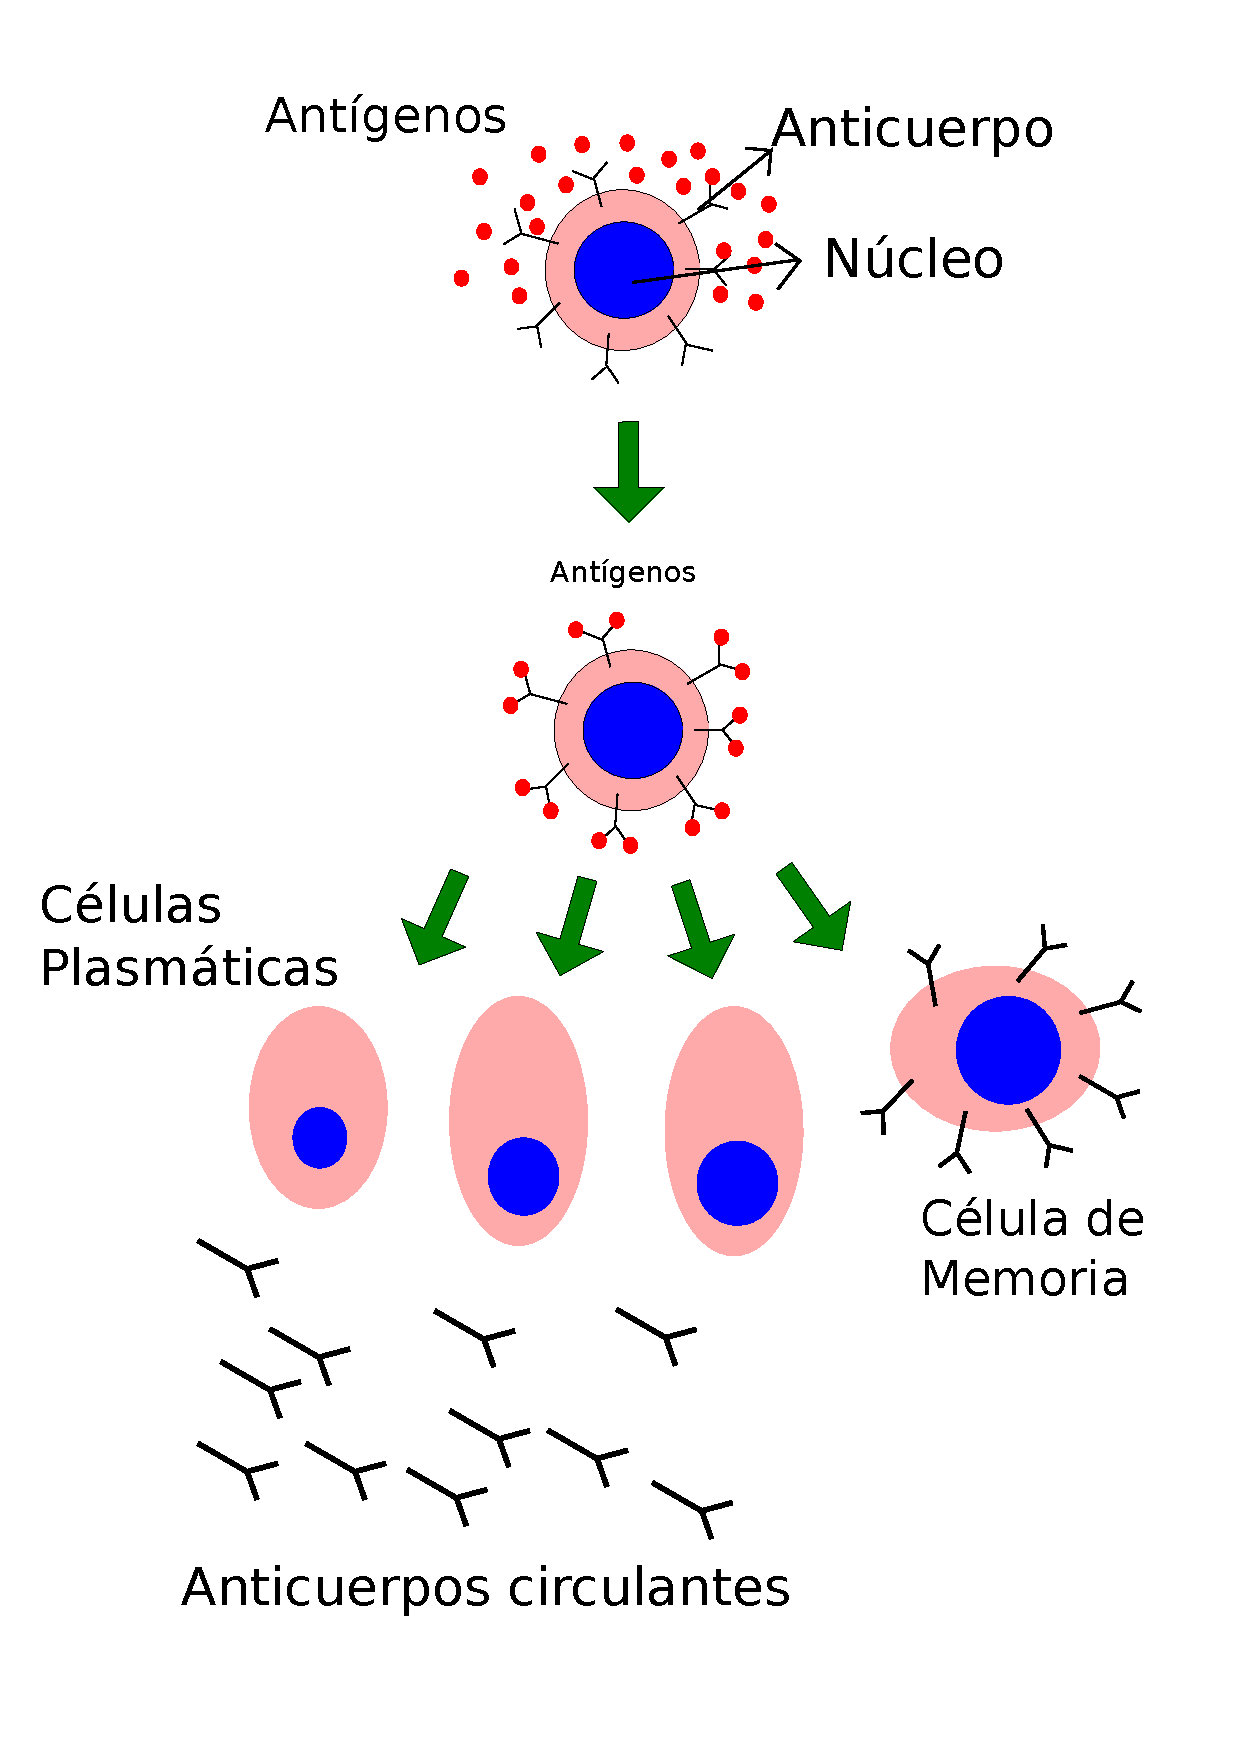
\includegraphics[width=0.5\textwidth]{img/clonalSelection.pdf}
\end{center}
\caption{Ejemplo de una selección clonal de linfocitos}
\label{fig:clonalSelection}
\end{figure}

Se señala la descripción de la figura~\ref{fig:clonalSelection} se detalla a continuación:

La teoría de la selección clonal de los anticuerpos indica que un linfocito B immaduro
se activa frente a la exposición de los antígenos, su posterior diferenciación en células
plasmáticas que sintetizan anticuerpos específicos en contra del antígeno y células de memoria.


\subsection{Algoritmo de la Selección Clonal}

Siguiendo el principio de selección clonal y el proceso de maduración de la afinidad, postulado por De Castro~\cite{decastro} se puede describir el algoritmo de selección clonal de la siguiente forma:
\begin{figure}[h!]
\begin{center}
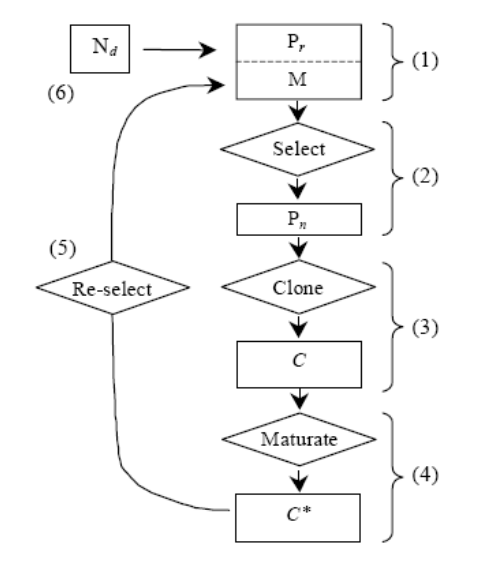
\includegraphics[width=0.5\textwidth]{img/algoritmo}
\end{center}
\caption{Diagrama del algoritmo de la selección clonal}
\label{fig:algoritmo}
\end{figure}

Siendo la explicación de los pasos de la figura~\ref{fig:algoritmo} la siguiente:
\begin{enumerate}
    \item Generar un conjunto (P) de soluciones candidatas, compuesto de células de memoria (M) añadidas a la población restante (Pr), teniendo entonces $P = Pr + M$
    \item Determinar los $n$ mejores individuos (Pn) de la población (P), basado en una medida de afinidad.
    \item Clonar (reproducir) estos $n$ mejores individuos de la población proporcional a su fitness, dando origen a una población temporal de clones (C).
    \item Someter la población de clones a un esquema de hiper-mutación (inversamente proporcional a la afinidad del anticuerpo). Una población de anticuerpos maduros es generada (C*).
    \item Seleccionar nuevamente los mejores individuos de (C*) para componer el conjunto de memoria. (Algunos reemplazos desde (C*) a (P), debido a la mejora)
    \item Reemplazar los $d$ anticuerpos con menor afinidad de la población, manteniendo la diversidad.
\end{enumerate}



\subsection{Estado del Arte Técnica}
\label{sec:estadoArteTecnica}
%Descripción de otras experiencias similares a la que se estudiará.
%Esta sección deberá contener la descripción de experiencias con el mismo problema/técnica
%(las mejores) o para problemas similares que puedan ayudarle como refrencia para su propuesta.

Desde que De Castro et al. publicó su trabajo \emph{`` Learning and optimization using clonal selection principle''}~\cite{decastro},
distintos investigadores se han dedicado a poder utilizar dicha teoría para implementar algoritmos que buscan
optimizar una tarea determinada, de hecho, la mayoría de los trabajos se centran en por ejemplo la \emph{optimización
de funciones}, \emph{optimización multiobjetivo}, sin dejar de lado los problemas típicos de optimización como lo son
\emph{path planning}, \emph{graph coloring}, \emph{vehicle routing}, \emph{entrenamiento de sistemas}, \emph{clasificadores},
\emph{reconocimiento de patrones}, etc, pero la presente sección se centra netamente en problemas abordados que puedan
tener una cierta relación a nivel de modelamiento, objetivos o tratamiento con el problema principal del presente trabajo,
el \emph{Car Sequencing Problem}.\\


% Clonal Selection based Mobile Robot Path Planning

Respecto al área de la robótica, Xuanzi Hu~\cite{robotPlanning} a podido dar un enfoque a las problemáticas relacionadas
con el \emph{Mobile Robot Path Planning}, realizando una comparativa con los algoritmos genéticos, en los cuales queda demostrado
la eficiencia y superioridad de la selección clonal, ya que al ser dos metodologías generacionales, se basan en los mismo principios,
y son fácilmente comparables al momento de realizar un \emph{benchmark} de ambas técnicas con parámetros lo más similar posible.
Una característica especial de la presente implementación son sus operadores inmunes utilizados, en los que están el operador de mutación
que consiste en elegir aleatoriamente un nodo del camino y reemplazarlo por otro nodo que no está en el camino original; el operador
de inserción, que se utiliza para poder reparar los segmentos de un camino infactible, insertando un nodo entre el problema y por último
el operador de supresión, que se aplica a los caminos factibles e infactibles. 

Un punto importante en éste trabajo es que a nivel de programación algorítmica, la selección clonal presenta una superioridad también,
al poder ser un algoritmo mucho más sencillo de  implementar que un algoritmo genético.\\
%%


% Scheduling Aircraft Landing Based on Clonal Selection Algorithm and Receding Horizon Control
Por otro lado Xiaolan Jia et al.~\cite{aircraft} utiliza la selección clonal hibridamente en conjunto con un modelo
de control predictivo llamado \emph{Receding Horizon Control (RHC)} para abordar el conocido problema de \emph{Scheduling Aircraft Landing},
en el cual la selección clonal forma parte del algoritmo RHC, ocupándose de realizar el scheduling propiamente tal.

Detalladamente las dos aproximaciones que plantea el presente trabajo de X. Jia, señala que una selección clonal con restricciones
basado en ``grados de infactibilidad'' (IFD) programa los aviones en el \emph{receding horizon} actual, en cambio
el RHC repite el proceso de optimización usando ``propagación de segmentos excelentes de genes'' (EGSS) hasta que todos los aviones
han aterrizado.

IFD maneja las restricciones de una buena manera y guía el proceso de optimización de manera efectiva,
por otro lado EGSS mejora la velocidad de convergencia del algoritmo, demostrando empíricamente que la aproximación con RHC
soluciona el problema de una manera mas efectiva y rápida.\\
%%


% Clonal Selection Algorithm for Vehicle Routing

Otro problema de optimización conocido como \emph{Vehicle Routing Problem (VRP)} ha sido atacado utilizando la selección clonal
también por varios autores, entre ellos destaca Jacek Dabrowski~\cite{vrp} pues soluciona una pequeña variación del
problema en conjunto llamado \emph{Capacitated Vehicle Routing Problem (CVRP)} en el cual una flota fija de vehículos de repartición
con una capacidad uniforme debe atender la demanda de un cliente determinado para un solo producto de un sólo almacén, cumpliendo
obviamente el mínimo costo de transito. Por lo que la única variación entre CVRP y VRP es que el primero añade la restricción
de que todos los vehículos deben tener una capacidad uniforme de un sólo producto.

Dabrowski señala que la selección clonal es una buena herramienta para la búsqueda de caminos múltiples,
ya que cuando entregamos una instancia del programa se puede un conjunto de soluciones como un conjunto de anticuerpo,
rankeando las soluciones mediante ``operadores de comparación'' y pero que existe un control sobre el ``operador de mutación''
entre los cuales están; EXC, que elige esquinas del camino y las trata de unir; SUM, que intenta concatenar dos rutas sin violar
restricciones; NEW, que construye nuevas ruta utilizando la heurística \emph{greedy} a partir de un vértice aleatorio.

Finalmente el único problema es que el autor señala que sería correcto realizar un benchmark con otras técnicas,
para poder comprobar que tan efectiva es la técnica.\\
%%


% Stretching Technique-based Clonal Selection Algorithm for Flexible Job-shop Scheduling
Como ya se vio anteriormente, en muchas investigaciones se utiliza la mezcla entre la selección clona y otra técnica,
y es el mismo casi que propone Lu Hong~\cite{jobshop} al utilizar una técnica de \emph{Stretching} al resolver
una variación del \emph{Job-shop scheduling problem (JSP)} llamado \emph{Flexible Job-shop Scheduling Problem (FJSP)},
la cual solo posee una mayor disponibilidad de máquinas para realizar las operaciones, es decir, sigue la dinámica
de encontrar una ubicación de cada operación y definir las secuencias de éstas en cada máquina, tratando de utilizar el mínimo
tiempo posible.

La técnica de \emph{stretching} fue propuesta por M. N. Vrahatis~\cite{stretching},
%M. Vrahatis, G. Androulakis and M. Manoussakis, “A new unconstrained optimization method for Imprecise function andgradient values,”
%Journal of Mathematical Analysis and Applications, 1996, pp. 586–607.
y su idea principal es realizar dos etapas de transformación sobre la forma de la función objetivo,
basada en la información de los mínimos locales, es decir, si hay un mínimo se busca realizando un algoritmo
de optimización convencional, y cuando se encuentra, la función objetivo se ``estira'' de acuerdo a unas expresiones determinadas.

Utilizando la función de \emph{stretching} no se cambian los objetivos buscando, pero provee una forma de escape
de los óptimos locales mejorando la convergencia global.

Generalmente luego de los test, STCSA muestra ser mejor que una selección clonal normal,
siendo una excelente aproximación para resolver problemas a larga escala cuando otros algoritmos fallan dando buenas soluciones.\\
%%


% Immune Clonal Selection Algorithm for Hybrid Flow-shop Scheduling Problem
Feng Liu et al.~\cite{flowshop} para poder reducir la complejidad computacional del
\emph{Hybrid Flow-shop Scheduling Problem} utiliza selección clonal.

Éste problema es una aplicación importante en las empresas manufactureras, ya que es un problema NP-completo,
y actualmente las tecnologías de optimización y algunas heurísticas como \emph{branch and bound}, \emph{genetic algorithm}
han sido utilizadas pero sin tanto éxito, ya que tienen distintos inconvenientes al momento de trabajar con problemas
de alto tamaño.

Liu realiza ésta elección, pues la selección clonal propone mecanismos especiales como la habilidad de mantener la diversidad
de los anticuerpos, mecanismos de auto-adaptación y funciones de memoria. Además para mejorar la exploración y explotación
se agrupan estrategias y operadores de multi-mutación (mutación clonal, cruzamiento clonal y selección clonal).\\
%%


% Computer Experiments with a Parallel Clonal Selection Algorithm for the Graph Coloring Problem
Finalmente, existen trabajos dignos de destacar, como la aproximación que entrega Jacek Dabrowski~\cite{graph}
al realizar experimentos con selección clonal pero utilizando conceptos de paralelismo para un problema básico como lo es
el \emph{Graph Coloring Problem}, comparandolo contra un algoritmo \emph{Tabu search} en paralelo.

Los anticuerpos son inicializados utilizando una asignación aleatorias de colores o utilizando una heurística \emph{greedy},
por otro lado, la selección clonal se enfoca a minimizar la función objetivo, siendo ésta el numero de conflictos de colores.

El mecanismo de hiper-mutación cambia la asignación de colores a los vértices del gráfico.

Para mejorar el desempeño de la versión paralela que se ha creado se utilizada el modelo de ``isla'' (asincrónico),
donde cada procesador trabaja con su propio conjunto de anticuerpos.

Lo llamativo surge al existir mecanismos de ``migración'' que permite un intercambio de conocimiento entre los 
distintos procesos, los cuales son elegidos mediante una ``selección de torneo''.

Por lo tanto la selección clonal se sobrepone a \emph{Tabu search} en todas las instancias,
llegando a la conclusión que aunque no posea un operador de cruzamiento, la selección clonal
es una forma fácil de implementar un algoritmo de optimización.
%%

Con respecto a los componentes que cada implementación revisada proponen, podemos decir que algunos procedimientos
van a depender netamente con el tipo de problema que queremos resolver. Una de las formas es poder implementar
una suerte de \emph{operadores inmunes} los cuales nos pueden servir para insertar diversidad a nuestra población,
reparar poblaciones poco beneficiosas y finalmente el aspecto de mutación, para poder obtener nuestra nueva
población.
Otra forma explicada en un trabajo revisado, es la implementación de un \emph{operador de comparación}, que va
a tener relación con un ranking a cada solución obtenida.
Siguiendo con los buenos componenetes, al momento de ingresar diversidad a nuestra población, varios investigadores
lo hacen generando soluciones aleatorias, pero éste proceso podría ser mejorando utilizando técnicas como Greedy.


Finalmente los algoritmos inmunes, en especial los algoritmos de ``selección clonal'' suelen ser una buena aproximación
para poder solucionar problemas de optimización y gracias a los estudios analizados en el estado del arte del problema,
podemos decir que es una buena solución para el ``Car Sequencing Problem''.



\section{Bibliografía}
%Se debe referenciar todo paper citado. En caso de referenciar páginas web, debe incluir fecha.
\bibliography{informe}
\end{document} 
